
\section{Rückblick}

\begin{frame}
  {Wortklassen: Grundlagen}
  \pause
  \begin{itemize}[<+->]
    \item Wortklassen als \alert{Grundausstattung der Grammatik}
    \item Vehikel für klassenbezogene Generalisierungen
    \item Bedeutung? --- nicht alle Wörter
      \Zeile
    \item Wortform\slash syntaktisches Wort:
      \begin{itemize}[<+->]
        \item konkrete Form \alert{im syntaktischen Kontext}
        \item voll spezifiziert (Merkmale, Werte)
      \end{itemize}
      \Zeile
    \item Wort\slash lexikalisches Wort:
      \begin{itemize}[<+->]
        \item abstrakte Form \alert{im Lexikon}
        \item evtl.\ unterspezifiziert
      \end{itemize}
      \Zeile
    \item "`Schulwortarten"': \alert{unzureichend operationalisiert}
  \end{itemize}
\end{frame}

% \begin{frame}
%   {Wortklassen: konkret}
%   \pause
%   \begin{itemize}[<+->]
%     \item morphologische Klassifikation: mögliche Paradigmen (Formen)
%     \item syntaktische Klassifikation: mögliche Syntagmen (Kontexte)
%      \Halbzeile 
%     \item \alert{Filtermethode}: Entscheidungsfragen zur Gliederung des Wortschatzes
%       \Halbzeile
%     \item flektierbare Wörter: Numerus, \alert{strukturell motiviert}
%     \item Substantive vs.\ Nomina: festes Genus
%     \item Adjektive: Stärkeflexion
%     \item Präpositionen: Kasusrektion, einstellige Valenz
%     \item Komplementierer: Einleitung von Verb-Letzt-Satz
%     \item Adverben vs.\ Partikel: Vorfeldfähigkeit
%       \Halbzeile
%     \item Wortklassen insgesamt: \alert{nach unseren Anforderungen}
%     \item umfassende Systemkenntnis erforderlich (leichte Zirkularität)
%   \end{itemize}
% \end{frame}

\section{Überblick}

\begin{frame}
  {Morphologie: Flexion und Wortbildung}
  \pause
  \begin{itemize}[<+->]
    \item \alert{Formveränderungen} und \alert{Merkmalsänderungen}
      \begin{itemize}[<+->]
        \item Veränderungen von Werten
        \item Veränderungen von Merkmalsaustattungen
      \end{itemize}
      \Halbzeile
    \item Morphe und ihre Funktionen
    \item Morphe: nicht-lexikalische Morphe und Stämme
    \item Umlaut und Ablaut (bzw.\ Vokalstufen)
    \item statische und volatile Merkmale
    \item Wortbildung vs.\ Flexion, definiert anhand von Merkmalen
  \end{itemize}
\end{frame}

\begin{frame}
  {Morphologie und Bildungssprache\slash Normsprache}
  \pause
  \begin{itemize}[<+->]
    \item Flexion und zugehörige Funktionskategorien
      \begin{itemize}[<+->]
        \item normsprachlich überwiegend \alert{klar definiert}
        \item vorliterate perfekte Beherrschung nicht voraussetzbar (z.\,B.\ Konjunktiv)
          \Halbzeile
        \item erhebliche Abweichungen in \alert{Dialekten}, \alert{Soziolekten} und \alert{Kiezsprachen}
          \Halbzeile
        \item \textit{Et rēchnet aufe Terasse.} (Pott)
        \item Aber wie funktioniert das eigentlich genau?
          \Halbzeile
        \item \textit{Ich las schon einmal Rilke.} (rhfr. Hyperkorrektur)
        \item Im Odenwald gibt es kein Präteritum, wird in der Schule gelernt.
      \end{itemize}
     \Halbzeile 
    \item Wortbildung
      \begin{itemize}[<+->]
        \item wichtiger Kern der Bildungssprache (besonders Komposition)
          \Halbzeile
        \item \textit{Das ist wegen der Spannendheit.} (Kind, 7--8 Jahre, ca. 1992)
        \item \textit{Die Vase ist vollansichtlich reliefiert.} (Heide Rezepa-Zabel, 2018)
      \end{itemize}
  \end{itemize}
\end{frame}

\begin{frame}
  {Morphosyntax in der Schule}
  \pause
  Wozu ist so ein Unterricht gut?
  \pause
  \begin{center}
    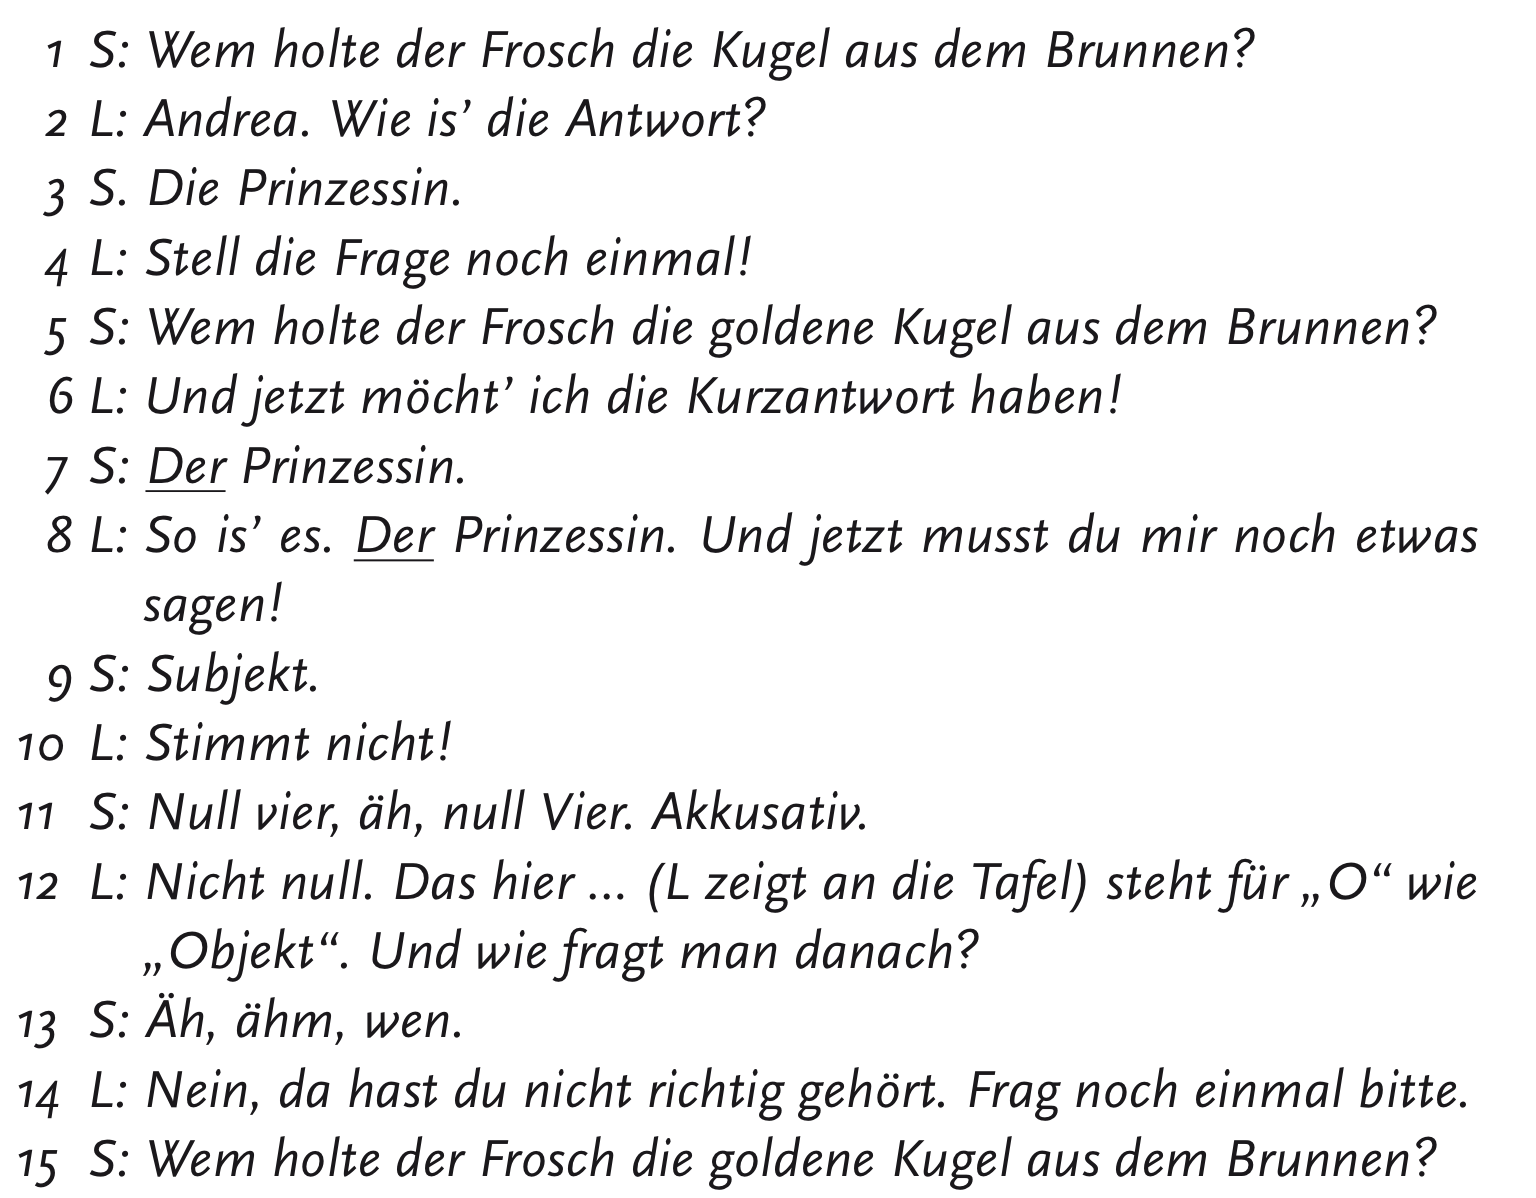
\includegraphics[width=0.6\textwidth]{graphics/kasusschule1}
  \end{center}
  \tiny \citet[36--37]{Gramzowemden2002}, zitiert nach \citet[257--258]{Bredel2013}
\end{frame}

\begin{frame}
  {Morphosyntax in der Schule}
  Wozu ist so ein Unterricht gut?
  \begin{center}
    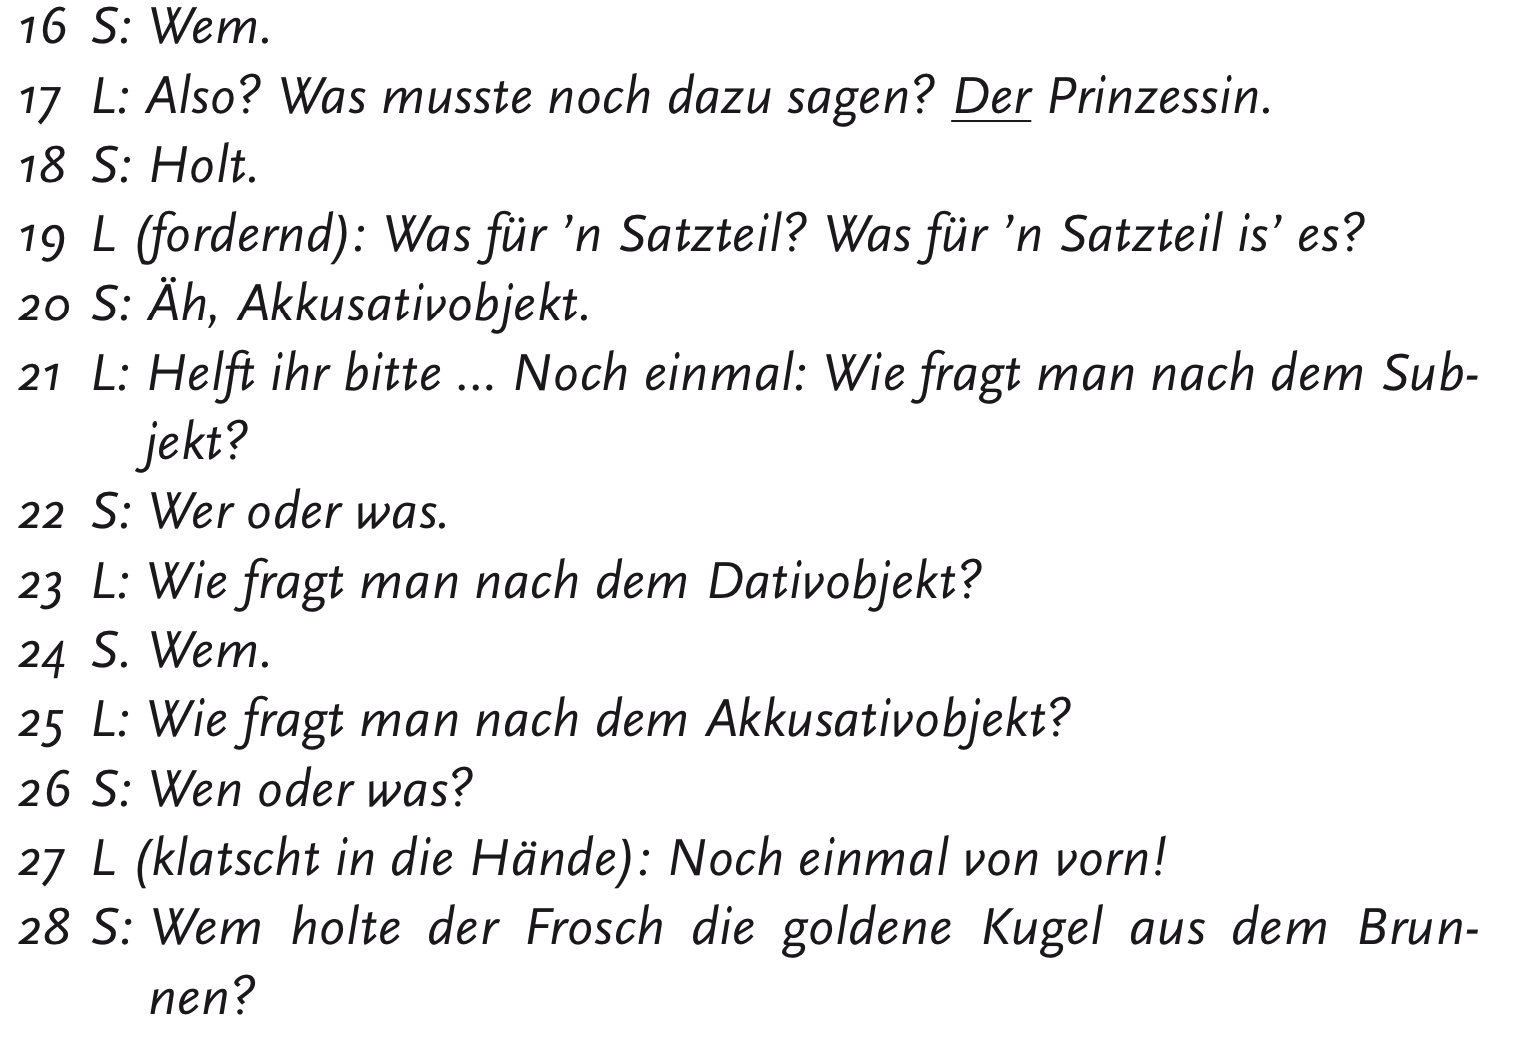
\includegraphics[width=0.6\textwidth]{graphics/kasusschule2}
  \end{center}
  \tiny \citet[36--37]{Gramzowemden2002}, zitiert nach \citet[257--258]{Bredel2013}
\end{frame}

\begin{frame}
  {Morphosyntax in der Schule}
  Wozu ist so ein Unterricht gut?
  \begin{center}
    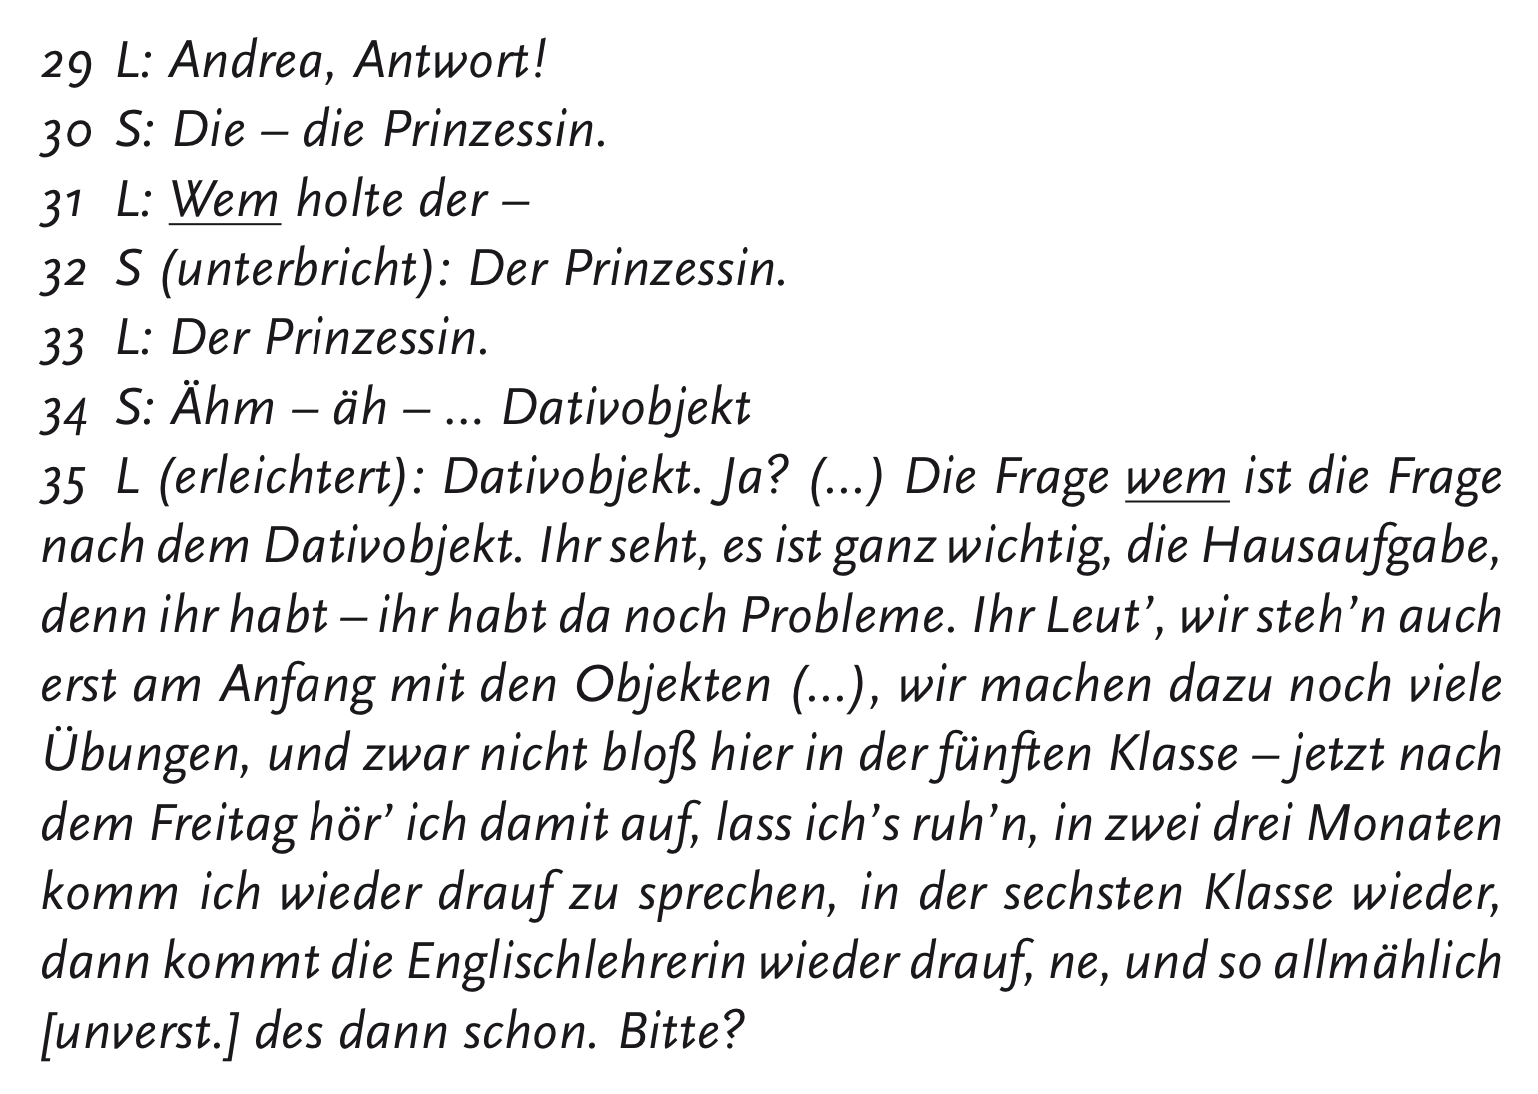
\includegraphics[width=0.6\textwidth]{graphics/kasusschule3}
  \end{center}
  \tiny \citet[36--37]{Gramzowemden2002}, zitiert nach \citet[257--258]{Bredel2013}
\end{frame}

\section{Morphologie}

\begin{frame}
  {Form und Funktion: Flexion}
  \pause
  \begin{exe}
    \ex
    \begin{xlist}
      \ex \alert{Den Präsidenten} begrüßte \alert{der Dekan} äußerst respektlos.
      \pause
      \ex \alert{Der Dekan} begrüßte \alert{den Präsidenten} äußerst respektlos.
    \end{xlist}
    \pause
    \ex
    \begin{xlist}
      \ex \alert{Die Präsidentin} begrüßte \alert{die Dekanin} äußerst respektlos.
      \pause
      \ex \alert{Die Dekanin} begrüßte \alert{die Präsidentin} äußerst respektlos.
    \end{xlist}
  \end{exe}
  \pause
  \Zeile
  Formveränderungen lexikalischer Wörter \alert{schränken ihre möglichen grammatischen Funktionen und Relationsbeziehungen im Satz ein}\dots\\
  \pause
  \Halbzeile
  \dots und sie haben semantische und systemexterne Folgen.

\end{frame}

\begin{frame}
  {Form und Funktion: Wortbildung}
  \pause
  \begin{exe}
    \ex grün\alert{lich}, röt\alert{lich}, gelb\alert{lich}
    \pause
    \ex Neu\alert{igkeit}, Blöd\alert{heit}, Tauch\alert{er}, Heb\alert{ung}
    \pause
    \ex Fensterh\alert{rahmen}, Tücher\alert{spender}, Glas\alert{korken}, Unter\alert{schrank}
  \end{exe}
  \pause
  \Zeile
  Formveränderungen von einem zu einem anderen lexikalischen Wort führen zu Bedeutungs- und kategorialen Veränderungen.
\end{frame}

\begin{frame}
  {Markierungsfunktionen von Morphen I}
  \pause
  \begin{exe}
    \ex
    \begin{xlist}
      \ex{(der) \alert<4>{Berg}}
      \ex{(den) \alert<4>{Berg}}
      \ex{(dem) \alert<4>{Berg}}
      \ex{(des) \alert<5>{Berg}\rot<5>{-es}}
      \ex{(die) \alert<6>{Berg}\rot<6>{-e}}
      \ex{(der) \alert<6>{Berg}\rot<6>{-e}}
    \end{xlist}
    \pause
    \ex
    \begin{xlist}
      \ex{(der) \alert<8>{Mensch}}
      \ex{(den) \alert<9>{Mensch}\rot<9>{-en}}
      \ex{(dem) \alert<9>{Mensch}\rot<9>{-en}}
      \ex{(des) \alert<9>{Mensch}\rot<9>{-en}}
      \ex{(die) \alert<9>{Mensch}\rot<9>{-en}}
      \ex{(der) \alert<9>{Mensch}\rot<9>{-en}}
    \end{xlist}
  \end{exe}
\end{frame}

\begin{frame}
  {Markierungsfunktionen von Morphen II}
  \pause
  \begin{exe}
    \ex
    \begin{xlist}
      \ex{(ich) \alert<3>{kauf}\rot<3>{-e}}
      \ex{(du) \alert<4>{kauf}\rot<4>{-st}}
      \ex{(wir) \alert<5>{kauf}\rot<5>{-en}}
      \ex{(sie) \alert<5>{kauf}\rot<5>{-en}}
    \end{xlist}
  \end{exe}
\end{frame}

\begin{frame}
  {Morphe und Markierungsfunktionen}
  \pause
  \begin{itemize}[<+->]
    \item Formveränderungen:
      \begin{itemize}[<+->]
        \item oft nicht \alert{eine} Funktion
        \item \rot{Einschränkung} der möglichen Funktionen
      \end{itemize}
   \Halbzeile 
    \item \alert{Markierungsfunktion}: eine \alert{Reduktion}\\
      der möglichen Merkmale oder Werte einer Wortform
    \item zum Beispiel \textit{-en} bei schw.\ Maskulina: \rot{nicht} Nominativ Singular
    \item oder \textit{-en} bei Verben im Präsens: Plural und nicht adressatbezogen
      \Halbzeile
    \item (Extremfall der Einschränkung entspricht einer positiven Spezifikation)
      \Halbzeile
    \item \alert{Morphe = alle segmentalen Einheiten mit Markierungsfunktion}
  \end{itemize}
\end{frame}

\begin{frame}
  {Stämme I}
  \pause
  \begin{exe}
    \ex
    \begin{xlist}
      \ex{(ich) \alert<5->{kauf}-e\\
        (du) \alert<5->{kauf}-st\\
        (ihr) \alert<5->{kauf}-t }
        \pause
        \ex{(ich) \alert<6->{kauf}-te\\
        (du) \alert<6->{kauf}-test\\
        (ihr) \alert<6->{kauf}-tet}
        \pause
        \ex{(ich habe) ge-\alert<7->{kauf}-t\\
        (du hast) ge-\alert<7->{kauf}-t\\
        (ihr habt) ge-\alert<7->{kauf}-t}
    \end{xlist}
  \end{exe}
\end{frame}

\begin{frame}
  {Stämme II}
  \begin{exe}
    \ex
    \begin{xlist}
      \ex{(ich) \alert<4->{nehm}-e\\
        (du) \rot<5->{nimm}-st\\
          (es) \rot<5->{nimm}-t\\
          (ihr) \alert<4->{nehm}-t}
        \pause
        \ex{(ich) \orongsch<6->{nahm}\\
        (du) \orongsch<6->{nahm}-st\\
          (ihr) \orongsch<6->{nahm}-t}
        \pause
        \ex{(ich habe) ge-\gruen<7->{nomm}-en\\
        (du hast) ge-\gruen<7->{nomm}-en\\
        (ihr habt) ge-\gruen<7->{nomm}-en}
    \end{xlist}
  \end{exe}
  \pause
  \pause
  \pause
  \pause
  \pause
  Der \alert{Stamm} kann nicht "`der unveränderliche Wortbestandteil"'\\
  eines lexikalischen Wortes (in einem Paradigma) sein.\\
  \Zeile
  \pause
  \alert{\dots aber der mit der Bedeutung, also der} \rot{lexikalischen Markierungsfunktion}!
\end{frame}

\begin{frame}
  {Affixe}
  \pause
  \begin{exe}
    \ex
    \begin{xlist}
      \ex (ich) nehm\alert<6->{-e}
      \pause
      \ex (des) Berg\alert<7->{-es}
      \pause
      \ex Schön\alert<8->{-heit}
      \pause
      \ex \alert<9->{Un-}ding
    \end{xlist}
  \end{exe}
  \Zeile
  \pause
  \pause
  \pause
  \pause
  \pause
  \begin{itemize}[<+->]
    \item \alert{keine lexikalische Markierungsfunktion}
    \item \alert{nicht wortfähig} = nicht ohne Stamm verwendbar
  \end{itemize}
\end{frame}

\begin{frame}
  {Umlaut vs.\ Ablaut: Warum erst jetzt?}
  \pause
  \alert{"`So ein chaotisches Buch! Plötzlich geht es\\
  in der Morphologie wieder um Phonologie!"'}\pause --- Ja\dots
  \pause
  \Zeile
  \begin{itemize}[<+->]
    \item Morphophonologie
    \item Morphosyntax
    \item Syntax-Semantik-Schnittstelle
    \item Prosodie-Pragmatik-Schnittstelle
    \item usw.
      \Zeile
    \item \rot{Die Grammatik nutzt die verfügbaren Mittel gut aus,\\
      und Markierungsmöglichkeiten aller Ebenen können\\
    auf anderen Ebenen zum Einsatz kommen.}
  \end{itemize}
\end{frame}

\begin{frame}[fragile]
  {Umlaut: Beschreibung}
  \pause
  \begin{center}
    \resizebox{0.4\textwidth}{!}{
    \begin{tikzpicture}[scale=3.5,baseline=default]
      \large
      \tikzset{
        vowel/.style={fill=white, anchor=mid, text depth=0ex, text height=1ex},
        vowelgespannt/.style={circle,fill=gray!30, anchor=mid, text depth=0ex, text height=1ex,minimum size=4ex},
        dot/.style={circle,fill=black,minimum size=0.4ex,inner sep=0pt,outer sep=-1pt},
      }

      \coordinate (hf) at (0,2); % high front
      \coordinate (hb) at (2,2); % high back
      \coordinate (lf) at (1,0); % low front
      \coordinate (lb) at (2,0); % low back
      \def\V(#1,#2){barycentric cs:hf={(3-#1)*(2-#2)},hb={(3-#1)*#2},lf={#1*(2-#2)},lb={#1*#2}}

      % Chart key (vorne -- hinten).
      \draw [{Latex[round]}-] (\V (-.25,0)) -- (\V (-.25,.5)) node[above left] {\footnotesize vorne};
      \draw [-{Latex[round]}] (\V (-.25,1.5)) -- (\V (-.25,2)) node[above left] {\footnotesize hinten};
      \path (\V (-.25,1)) node[above] {\footnotesize zentral};

      % Chart key (hoch -- tief).
      \draw [{Latex[round]}-] (\V (0,-.25)) -- +(270:.5cm) node[above right,rotate=90] (vokaltrapez1) {\footnotesize hoch};
      \draw [{Latex[round]}-] (\V (3,-2.5)) -- +(270:-.5cm) node[above left,rotate=90] (vokaltrapez2) {\footnotesize tief};
      \path (\V (1.5,-1)) node[above,rotate=90] {\footnotesize mittel};

      % Grid.
      \draw [gray, thick] (\V(0,0)) -- (\V(0,2));
      \draw [gray, thick] (\V(3,0)) -- (\V(3,2));
      \draw [gray, thick] (\V(0,0)) -- (\V(3,0));
      \draw [gray, thick] (\V(0,2)) -- (\V(3,2));

      % Vowels.
      \path (\V (0,2))     node[vowelgespannt] (u)   {u};
      \path (\V(0,0))      node[vowelgespannt] (y)   {y};
      \path (\V (0.5,1.5)) node[vowel]         (uu)  {ʊ};
      \path (\V(0.5,0.5))  node[vowel]         (yy)  {ʏ};
      \path (\V (1,2))     node[vowelgespannt] (o)   {o};
      \path (\V(1.25,0))   node[vowelgespannt] (oe)  {ø};
      \path (\V(3,1))      node[vowelgespannt] (a)   {a};
      \path (\V(2,0))      node[vowelgespannt] (ee)  {ɛ};
      \path (\V(2.5,1))    node[vowel]         (aa)  {ă};
      \path (\V(1.65,0.5)) node[vowel]         (eee) {ɛ̆};
      \path (\V (1.5,1.4)) node[vowel]         (oo)  {ɔ};
      \path (\V(1.4,0.5))  node[vowel]         (oee) {œ};

      \only<3>{\path (u)  edge [-{Latex[round]}, bend left=10]  (y);}
      \only<4>{\path (uu) edge [-{Latex[round]}, bend left=10]  (yy);}
      \only<5>{\path (o)  edge [-{Latex[round]}, bend right=10] (oe);}
      \only<6>{\path (oo) edge [-{Latex[round]}, bend right=5]  (oee);}
      \only<7>{\path (aa) edge [-{Latex[round]}, bend right=10] (eee);}
      \only<8>{\path (a)  edge [-{Latex[round]}, bend left=10]  (ee);}
      
      \only<9->{\path (u)  edge [-{Latex[round]}, bend left=10]  (y);
        \path (uu) edge [-{Latex[round]}, bend left=10]  (yy);
        \path (o)  edge [-{Latex[round]}, bend right=10] (oe);
        \path (oo) edge [-{Latex[round]}, bend right=5]  (oee);
        \path (aa) edge [-{Latex[round]}, bend right=10] (eee);
        \path (a)  edge [-{Latex[round]}, bend left=10]  (ee);}
    \end{tikzpicture}
    }
  \end{center}
  \raggedleft
  \only<3>{G\rot{u}t [g\rot{uː}t] -- G\rot{ü}ter [g\rot{yː}tɐ]}
  \only<4>{M\rot{u}tter [m\rot{ʊ}tɐ] -- M\rot{ü}tter [m\rot{ʏ}tɐ]}
  \only<5>{T\rot{o}n [t\rot{oː}n]-- T\rot{ö}ne [t\rot{øː}nə]}
  \only<6>{\rot{o}ft [ʔ\rot{ɔ}ft] -- \rot{ö}fter [ʔ\rot{œ}ftɐ]}
  \only<7>{kr\rot{a}nk [kʁ\rot{a}ŋk] -- kr\rot{ä}nker [kʁ\rot{ɛ}ŋkɐ]}
  \only<8>{B\rot{a}d [b\rot{aː}t] -- B\rot{ä}der [b\rot{ɛ}dɐ]}
  \centering
  \onslide<9->{Ein vorhersagbarer Prozess: \alert{Frontierung!}}
\end{frame}

\begin{frame}[fragile]
  {Ablaut: Beschreibung?}
  \pause
  Eine kleine Auswahl der möglichen Ablautreihen\ldots
  \pause
  \begin{center}
    \resizebox{0.4\textwidth}{!}{
    \begin{tikzpicture}[scale=3.5,baseline=default]
      \large
      \tikzset{
        vowel/.style={fill=white, anchor=mid, text depth=0ex, text height=1ex},
        dot/.style={circle,fill=black,minimum size=0.4ex,inner sep=0pt,outer sep=-1pt},
      }

      \coordinate (hf) at (0,2); % high front
      \coordinate (hb) at (2,2); % high back
      \coordinate (lf) at (1,0); % low front
      \coordinate (lb) at (2,0); % low back
      \def\V(#1,#2){barycentric cs:hf={(3-#1)*(2-#2)},hb={(3-#1)*#2},lf={#1*(2-#2)},lb={#1*#2}}

      % Chart key (vorne -- hinten).
      \draw [{Latex[round]}-] (\V (-.25,0))   -- (\V (-.25,.5)) node [above left] {\footnotesize vorne};
      \draw [-{Latex[round]}] (\V (-.25,1.5)) -- (\V (-.25,2))  node [above left] {\footnotesize hinten};
      \path (\V (-.25,1)) node[above] {\footnotesize zentral};

      % Chart key (hoch--tief).
      \draw [{Latex[round]}-] (\V (0,-.25)) -- +(270:.5cm)  node [above right,rotate=90] (vokaltrapez1) {\footnotesize hoch};
      \draw [{Latex[round]}-] (\V (3,-2.5)) -- +(270:-.5cm) node [above left,rotate=90] (vokaltrapez2) {\footnotesize tief};
      \path (\V (1.5,-1)) node[above,rotate=90] {\footnotesize mittel};

      % Grid. 
      \draw [gray, thick] (\V(0,0)) -- (\V(0,2));
      \draw [gray, thick] (\V(1,0)) -- (\V(1,2));
      \draw [gray, thick] (\V(2,0)) -- (\V(2,2));
      \draw [gray, thick] (\V(3,0)) -- (\V(3,2));
      \draw [gray, thick] (\V(0,0)) -- (\V(3,0));
      \draw [gray, thick] (\V(0,1)) -- (\V(3,1));
      \draw [gray, thick] (\V(0,2)) -- (\V(3,2));

      % Unrounded-rounded pairs.
      \path (\V(0,0))     node [vowel] (i)   {i};
      \path (\V(0.5,0.5)) node [vowel] (I)   {ɪ};   
      \path (\V(1,0))     node [vowel] (e)   {e};
      \path (\V(2,0))     node [vowel] (E)   {ɛ};

      % Unpaired symbols.
      \path (\V(3,1))      node [vowel] (a)  {a};
      \path (\V (2,2))     node [vowel] (oo) {ɔ};
      \path (\V (1,2))     node [vowel] (o)  {o};
      \path (\V (0,2))     node [vowel] (u)  {u};
      \path (\V (0.5,1.5)) node [vowel] (uu) {ʊ};

      \only<4>{\path (i)  edge [red, *-{Latex[round, width=5pt]}, bend left=10] (o);}
      \only<5>{\path (e)  edge [cyan, *-{Latex[round, width=5pt]}, bend left=10] (o);}
      \only<6>{\path (I)  edge [blue, *-, bend right=10] (a);\path (a)  edge [blue, -{Latex[round, width=5pt]}, bend right=10] (uu);}
      \only<7>{\path (E)  edge [green, *-{Latex[round, width=5pt]}, bend right=10] (a);\path (a)  edge [green, -{Latex[round, width=5pt]}, bend right=10] (oo);}
      \only<8>{\path (a)  edge [brown, *-, bend right=10] (u);\path (u)  edge [brown, -{Latex[round, width=5pt]}, bend right=10] (a);}
      \only<9>{\path (u)  edge [orange, *-, bend right=10] (i);\path (i)  edge [orange, -{Latex[round, width=5pt]}, bend right=10] (u);}
      \only<10>{\path (I)  edge [purple, *-, bend left=10] (a);\path (a)  edge [purple, -{Latex[round, width=5pt]}, bend right=10] (E);}

      \only<11>{\path (i)  edge [red, *-{Latex[round, width=5pt]}, bend left=10] (o);
        \path (e)  edge [cyan, *-{Latex[round, width=5pt]}, bend left=10] (o);
        \path (I)  edge [blue, *-, bend right=10] (a);\path (a)  edge [blue, -{Latex[round, width=5pt]}, bend right=10] (uu);
        \path (E)  edge [green, *-{Latex[round, width=5pt]}, bend right=10] (a);\path (a)  edge [green, -{Latex[round, width=5pt]}, bend right=10] (oo);
        \path (a)  edge [brown, *-, bend right=10] (u);\path (u)  edge [brown, -{Latex[round, width=5pt]}, bend right=10] (a);
        \path (u)  edge [orange, *-, bend right=10] (i);\path (i)  edge [orange, -{Latex[round, width=5pt]}, bend right=10] (u);
        \path (I)  edge [purple, *-, bend left=10] (a);\path (a)  edge [purple, -{Latex[round, width=5pt]}, bend right=10] (E);}


    \end{tikzpicture}
    }
  \end{center}
  \raggedleft
  \only<4>{fr\textcolor{red}{ie}ren [fʁ\textcolor{red}{iː}ʁən] -- fr\textcolor{red}{o}r [fr\textcolor{red}{oː}͡ɐ] -- gefr\textcolor{red}{o}ren [gəfr\textcolor{red}{oː}ʁən]}
  \only<5>{h\textcolor{cyan}{e}ben [h\textcolor{cyan}{eː}bən] -- h\textcolor{cyan}{o}b [h\textcolor{cyan}{oː}p] -- geh\textcolor{cyan}{o}ben [gəh\textcolor{cyan}{oː}bən]}
  \only<6>{b\textcolor{blue}{i}nden [b\textcolor{blue}{ɪ}ndən] -- b\textcolor{blue}{a}nd [b\textcolor{blue}{a}nt] -- geb\textcolor{blue}{u}nden [gəb\textcolor{blue}{ʊ}ndən]}
  \only<7>{b\textcolor{green}{e}rgen [b\textcolor{green}{ɛ}͡əgən] -- b\textcolor{green}{a}rg [b\textcolor{green}{a}͡ək] -- geb\textcolor{green}{o}rgen [gəb\textcolor{green}{ɔ}͡əgən]}
  \only<8>{sch\textcolor{brown}{a}ffen [ʃ\textcolor{brown}{a}fən] -- sch\textcolor{brown}{u}f [ʃ\textcolor{brown}{uː}f] -- gesch\textcolor{brown}{a}ffen [gəʃ\textcolor{brown}{a}fən]}
  \only<9>{sch\textcolor{orange}{i}nden [ʃ\textcolor{orange}{ɪ}ndən] -- sch\textcolor{orange}{u}nd [ʃ\textcolor{orange}{ʊ}nt] -- gesch\textcolor{orange}{u}nden [gəʃ\textcolor{orange}{ʊ}ndən]}
  \only<10>{s\textcolor{purple}{i}tzen [z\textcolor{purple}{ɪ}t͡sən] -- s\textcolor{purple}{a}ß [z\textcolor{purple}{aː}s] -- ges\textcolor{purple}{e}ssen [gəz\textcolor{purple}{ɛ}sən]}
  \centering
  \onslide<11->{\rot{Kein vorhersagbarer Prozess!} Lexikalisch\slash verbklassenbasiert.}
\end{frame}

% \begin{frame}
%   {Strukturbildung auf allen Ebenen (Kapitel 2)}
%   \pause
%   \begin{exe}
%     \ex\label{ex:strukturbildung021}
%     \begin{xlist}
%       \ex \textbf{Satz} \\
%       {[Alexandra schießt den Ball ins gegnerische Tor.]}
%       \pause
%       \ex \textbf{Satzteile} \\
%       {[Alexandra] [schießt] [den Ball] [ins gegnerische Tor]}
%       \pause
%       \ex \textbf{Wörter} \\
%       {[Alexandra] [schießt] [den] [Ball] [ins] [gegnerische] [Tor]}
%       \pause
%       \ex \textbf{Wortteile} \\
%       {[Alexandra] [schieß][t] [den] [Ball] [ins] [gegner][isch][e] [Tor]}
%       \pause
%       \ex \textbf{Laute} \\
%       {[A][l][e][k][s][a][n][d][r][a] \ldots \\}
%     \end{xlist}
%   \end{exe}
%   \pause
%   \Halbzeile
%   \begin{itemize}[<+->]
%     \item Strukturbildung: lineare Verbindung von Einheiten
%     \item durch Wiederholung: \alert{geschachtelte} Struktur
%     \item \alert{Konstitutenten}: Einheiten, aus denen Strukturen bestehen
%   \end{itemize}
% \end{frame}
% 
% \begin{frame}
%   {Strukturbildung in der Morphologie: Lineare Kombination}
%   \pause
%   \begin{exe}
%     \ex
%     \begin{xlist}
%       \ex{Un-ding}
%       \pause
%       \ex{(ich) ver-misch(-e)}
%     \end{xlist}
%     \pause
%     \ex
%     \begin{xlist}
%       \ex{(ich) leb-e}
%       \pause
%       \ex{Gleich-heit}
%     \end{xlist}
%     \pause
%     \ex{Ge-red-e}
%   \end{exe}
% \end{frame}
% 
% \begin{frame}[fragile]
%   {Hierarchische Struktur in der Morphologie}
%   \pause
%   \begin{center}
%     \scalebox{0.7}{
%       \begin{forest}
%         [Wortform
%           [{[Wortform]}
%             [Stamm, tier=preterminal
%               [\textit{schick}]
%             ]
%             [Flexionssuffix, tier=preterminal
%               [\textit{te}]
%             ]
%           ]
%           [Flexionssuffix, tier=preterminal
%             [\textit{-n}]
%           ]
%         ]
%       \end{forest}
%     }~\pause\scalebox{0.7}{
%       \begin{forest}
%         [Wortform
%           [Stamm\Sub{2}
%             [Wortbildungspräfix, tier=preterminal
%               [\textit{ver-}]
%             ]
%             [Stamm\Sub{1}, tier=preterminal
%               [\textit{schenk}]
%             ]
%           ]
%           [Flexionssuffix, tier=preterminal
%             [\textit{-t}]
%           ]
%         ]
%       \end{forest}
%     }
%   \end{center}
%   \Zeile
%   \pause
%   Solche Hierarchien ergeben sich automatisch dadurch, dass wir\\
%   mehrfach (hintereinander) Einheiten aneinanderhängen.
% \end{frame}

\begin{frame}
  {Statische und volatile Merkmale, Wortbildung und Flexion}
  \pause
  \begin{itemize}[<+->]
    \item Eigenschaften: "`Rotsein"' (Erdbeere), "`325m hoch"' (Eiffelturm) usw.
    \item Merkmale: \alert{\textsc{Farbe}}, \alert{\textsc{Länge}} usw.
    \item Werte: \alert{\textit{rot}}, \alert{\textit{grau}}; \alert{\textit{3cm}}, \alert{\textit{325m}}
  \end{itemize}
  \pause
  \Zeile
  \begin{exe}
    \ex
    \begin{xlist}
      \ex{Haus = [\textsc{Bed}: \textbf{\textit{haus}}, \textsc{Klasse}: \textbf{\textit{subst}}, \textsc{Gen}: \textbf{\textit{neut}}, \textsc{Kas}: \textit{nom}, \textsc{Num}: \textit{sg}]}
      \pause
      \ex{Haus-es = [\textsc{Bed}: \textbf{\textit{haus}}, \textsc{Klasse}: \textbf{\textit{subst}}, \textsc{Gen}: \textbf{\textit{neut}}, \textsc{Kas}: \textit{gen}, \textsc{Num}: \textit{sg}]}
      \pause
      \ex{Häus-er = [\textsc{Bed}: \textbf{\textit{haus}}, \textsc{Klasse}: \textbf{\textit{subst}}, \textsc{Gen}: \textbf{\textit{neut}}, \textsc{Kas}: \textit{nom}, \textsc{Num}: \textit{pl}]}
    \end{xlist}
  \end{exe}
  \Zeile
  \pause
  \begin{itemize}[<+->]
    \item bei einem lexikalischen Wort:
      \begin{itemize}
        \item \alert{statische Merkmale} wertestabil
        \item \alert{volatile Merkmale} werteverändernd im Paradigma
      \end{itemize}
  \end{itemize}
\end{frame}

\begin{frame}
  {Eigenschaften von Wortbildung}
  \pause
  \begin{exe}
    \ex
    \begin{xlist}
      \ex trocken (Adj) → \alert{Trocken-heit} (Subst)
      \ex Kauf (Subst), Rausch (Subst) → \alert{Kauf-rausch} (Subst)
      \ex gehen (V) → \alert{be-gehen} (V)
    \end{xlist}
    \pause
    \ex
    \begin{xlist}
      \ex lauf-en (Inf) → \alert{lauf-e} (1 Sg Prs Ind)
      \ex Münze (Sg) → \alert{Münze-n} (Pl)
    \end{xlist}
  \end{exe}
  \pause
  \Halbzeile
  \begin{itemize}[<+->]
    \item \rot{statische Merkmale bei Wortbildung}
      \begin{itemize}[<+->]
        \item geändert (Wortklasse, Bedeutung)
        \item gelöscht (alles außer Bedeutung: Komposition)
        \item umgebaut (Valenz von Verben beim Applikativ)
      \end{itemize}
  \Halbzeile
    \item anders als bei Flexion:
      \begin{itemize}
        \item \alert{produktives Erschaffen neuer Wörter}
        \item semantisch\slash grammatisch oft eingeschränkt
        \item nicht immer affigierend
      \end{itemize}
  \end{itemize}
\end{frame}

\section{Funktionen der nominalen Flexionsmerkmale}

\begin{frame}
  {Was heißt Funktion?}
  \pause
  Rückgriff auf Kapitel 3:
  \pause
  \Halbzeile
  \begin{itemize}[<+->]
    \item \alert{externe} Funktion: kommunikativ, pragmatisch, textuell, kulturell, \dots
    \item \alert{interne} Funktion: innerhalb der Grammatik Relationen kennzeichnend,
      Rekonstruktion der Struktur ermöglichend, Schnittstelle zur Semantik: \rot{Kompositionalität}
    \item nicht immer trennbar
      \Halbzeile
    \item Paradebeispeil für interne Funktion: \alert{Kasussystem}
      \Halbzeile
    \item konstruktioneller Ikonismus \citep{Eisenberg2013a}: Modellierung\\
      des internen Funktionssystems parallel zu externen Funktionen
  \end{itemize}
\end{frame}

\begin{frame}
  {Nominalphrasen oder NPs (vorläufig)}
  \pause
  Vorgriff auf Kapitel 11 und 12\dots\\
  \pause
  \Halbzeile
  \begin{exe}
    \ex
    \begin{xlist}
      \ex{[Gewichtheberinnen] haben [ein hartes Trainingsprogramm].}
      \pause
      \ex{[Trainierte Gewichtheberinnen] haben [Chancen]\\auf [die Goldmedaille].}
      \pause
      \ex{[Eine hervorragende Gewichtheberin] wurde [Olympiasiegerin].}
    \end{xlist}
  \end{exe}
  \pause
  \begin{itemize}[<+->]
    \item \alert{Eine Nominalphrase (NP; vorläufige Definition) ist\\
      eine Struktur aus Nomina, die zusammen stehen,\\
      und die in Kasus, Numerus und Genus kongruieren.}
      \Halbzeile
    \item typische Muster:
      \begin{itemize}
        \item{[(Adjektiv) Substantiv\Sub{Plural}]}
        \item{[Artikel\slash Pronomen (Adjektiv) Substantiv]}
        \item{[Pronomen]}
      \end{itemize}
      \Halbzeile
    \item hier fehlen: Relativsätze, Komplementsätze, andere Kleinigkeiten
  \end{itemize}
\end{frame}

\begin{frame}
  {Numerus}
  \pause
  \begin{exe}
    \ex
    \begin{xlist}
      \ex[ ]{Die Trainerin beobachtet [einen guten Wettkampf].}
      \pause
      \ex[*]{Die Trainerin beobachtet [einen guten Wettkämpfe].}
    \end{xlist}
    \pause
    \ex
    \begin{xlist}
      \ex[ ]{Die Trainerin beobachtet [einige gute Wettkämpfe].}
      \pause
      \ex[*]{Die Trainerin beobachtet [einige gute Wettkampf].}
    \end{xlist}
  \end{exe}
  \pause
  \Halbzeile
  \begin{itemize}[<+->]
    \item \alert{Anzahl von Objekten ("`Gegenständen"')}: konzeptuell beim Subst motiviert
    \item notwendigerweise volatiles Merkmal beim Subst
    \item Pluraliatantum wie \textit{Ferien} oder Singulariatantum wie \textit{Gesundheit}
    \item statisches Merkmal nur bei manchen Pronomina\slash Artikeln\\
      (\textit{ein}, \textit{drei}, \textit{einige}, \textit{viele})
  \end{itemize}
\end{frame}

\begin{frame}
  {Kasus}
  \pause
  Was ist Kasus? Haben die Kasus eine Bedeutung?
  \Halbzeile
  \pause
  \begin{exe}
    \ex
    \begin{xlist}
      \ex{Wir sehen \alert<13->{den Rasen}.}
      \pause
      \ex{Wir begehen \alert<14->{den Rasen}.}
      \pause
      \ex{Wir säen \alert<15->{den Rasen}.}
      \pause
      \ex{Wir fürchten \alert<16->{uns}.}
    \end{xlist}
    \pause
    \ex
    \begin{xlist}
      \ex{Sarah backt \alert<17->{ihrer Freundin} einen Marmorkuchen.}
      \pause
      \ex{Wir kaufen \alert<18->{dir} ein Kilo Rohrzucker.}
      \pause
      \ex{Die Mannschaft spielt \alert<19->{mir} zu drucklos.}
      \pause
      \ex{Der Marmorkuchen schmeckt \alert<20->{den Freundinnen} gut.}
    \end{xlist}
    \pause
    \ex
    \begin{xlist}
      \ex \alert<21->{Nächsten März} fahre ich zum Bergwandern in die Tatra.
      \ex Es waren \alert<22->{den ganzen Tag} Menschen zum Gipfel unterwegs.
    \end{xlist}
    \pause
    \ex
    \begin{xlist}
      \ex Das Ferienhaus \alert<23->{einer Freundin} steht im Juni leer.
      \ex Der Kragen \alert<24->{der Jacke} \rot<25->{meiner Oma} ist dreckig.
    \end{xlist}
  \end{exe}
\end{frame}

\begin{frame}
  {Kasus: Eigenschaften}
  \pause
  \begin{center}
    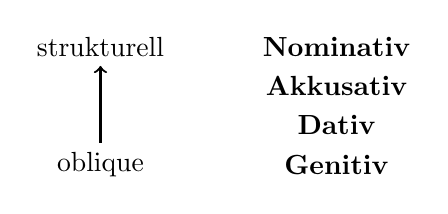
\begin{tikzpicture}
      \node (obl)                             {oblique};
      \node (gen) at ([shift={( 3,0)}]   obl) {\textbf{Genitiv}};
      \node (dat) at ([shift={( 0,0.5)}] gen) {\textbf{Dativ}};
      \node (akk) at ([shift={( 0,0.5)}] dat) {\textbf{Akkusativ}};
      \node (nom) at ([shift={( 0,0.5)}] akk) {\textbf{Nominativ}};
      \node (str) at ([shift={(-3,0)}]   nom) {strukturell};
      \draw [->, thick] (obl) to (str);
    \end{tikzpicture}

    \vspace{2\baselineskip}
    \pause
    \scalebox{0.8}{\begin{tabular}{lp{0.1cm}llll}
      \toprule
       \textbf{Eigenschaft} && \textbf{Nominativ} & \textbf{Akkusativ} & \textbf{Dativ} & \textbf{Genitiv} \\
      \hline
      verbregiert && fast immer & oft & oft & selten \\
      eigene Semantik && nein & fast nie & manchmal & manchmal \\
      attributiv && nein & nein & nein & ja \\
      präpositionsregiert && nie & oft & oft & oft \\
      \bottomrule
    \end{tabular}}
    \pause

    \vspace{2\baselineskip}
    \large \rot{Und Kasus kann nicht über Grammatikerfragen\\
    ("`Wen oder was?"' und so weiter) ermittelt werden!}
  \end{center}
\end{frame}

\begin{frame}
  {Person: Deixis}
  \pause
  Was ist die grammatische Person?

  \Halbzeile
  \pause
  \begin{exe}
    \ex
    \begin{xlist}
      \ex{Ich unterstütze den FCR Duisburg.}
      \pause
      \ex{Ihr unterstützt den FCR Duisburg.}
      \pause
      \ex{Sie/Diese/Jene/Eine/Man\ldots unterstützt den FCR Duisburg.}
      \pause
      \ex{Sie/Diese/Jene/Einige/\ldots unterstützen den FCR Duisburg.}
    \end{xlist}
  \end{exe}
  \pause
  \Halbzeile
  \begin{itemize}[<+->]
    \item prototypisch beim \alert{Pronomen} funktional motiviert
    \item Substantive: statisch dritte Person
      \Halbzeile
    \item hier: \rot{deiktische Pronomina}:
      \begin{itemize}[<+->]
        \item in einer Situation verweisend
        \item nur relativ zu einer Situation interpretierbar
      \end{itemize} 
  \end{itemize}
\end{frame}

\begin{frame}
  {Person: Anaphorik}
  \pause
  \begin{exe}
    \ex{\label{ex:person035}Sarah$_{\textnormal{1}}$ backt [ihrer Freundin]$_{\textnormal{2}}$ [einen Kuchen]$_{\textnormal{3}}$.\\
      Sie$_{\textnormal{1}}$ verwendet nur fair gehandelten unraffinierten Rohrzucker.}
      \pause
    \ex{\label{ex:person036}Sarah$_{\textnormal{1}}$ backt [ihrer Freundin]$_{\textnormal{2}}$ [einen Kuchen]$_{\textnormal{3}}$.\\
      Er$_{\textnormal{3}}$ besteht nur aus fair gehandelten Zutaten.}
      \pause
    \ex{\label{ex:person037}Sarah$_{\textnormal{1}}$ backt [ihrer Freundin]$_{\textnormal{2}}$ [einen Kuchen]$_{\textnormal{3}}$.\\
      Sie$_{\textnormal{2}}$ soll ihn$_{\textnormal{3}}$ zum Geburtstag geschenkt bekommen.}
  \end{exe}
  \Halbzeile
  \pause
  \begin{itemize}[<+->]
    \item \rot{anaphorische Pronomina}
    \item \alert{Rückverweis} im Text, Satz, Diskurs
    \item gleiche Indizes zeigen Bedeutungsidentität: \alert{Korreferenz}
  \end{itemize}
\end{frame}

\begin{frame}
  {Genus, Geschlecht, Gender?}
  \pause
  \begin{exe}
    \ex \label{ex:genus039}
    \begin{xlist}
      \ex{Die Petunie ist eine Blume.}
      \ex{Der Enzian ist eine Blume.}
      \ex{Das Veilchen ist eine Blume.}
    \end{xlist}
  \end{exe}
  \pause
  \Halbzeile
  \begin{itemize}[<+->]
    \item reine \alert{Subklassenbildung} beim Substantiv
    \item nicht in Geschlecht oder Gender motiviert
    \item tendentiell Korrespondenz von maskulin und männlich\\
      sowie feminin und weiblich
  \end{itemize}
\end{frame}

\section{Funktionen der Verbalflexion}

\begin{frame}
  {Rektion vs.\ funktionale Motivation:\\
  Numerus und Person der Verben}
  \pause
  \begin{itemize}[<+->]
    \item wie gezeigt wurde: \alert{Numerus} und \alert{Person}\\
      im Bereich der Nomina motiviert
    \item Subjekt-Verb-Kongruenz deshalb eher \alert{Rektion}? --- Nein.
      \Halbzeile
    \item Kongruenz:
      \begin{itemize}[<+->]
        \item reine \alert{Übereinstimmung von Werten}
        \item \rot{entsprechende Merkmale bei beiden Einheiten}
        \item Prototyp im Deutschen: \alert{Kongruenz innerhalb der NP}
      \end{itemize}
      \Halbzeile
    \item Rektion:
      \begin{itemize}[<+->]
        \item \alert{Merkmalsforderung} einer Einheit an die andere
        \item Regens: \rot{ohne} das regierte Merkmal
        \item Prototyp (im Deutschen): \alert{Kasusrektion} (der V und Prp)
      \end{itemize}
  \end{itemize}
\end{frame}

\begin{frame}
  {Tempus: synthetisch vs.\ analytisch}
  \pause
  Die klassischen "`Tempusformen"' des Deutschen:\\
  \Halbzeile
  \pause
  \begin{center}
    \scalebox{0.75}{\begin{tabular}{ll}
      \toprule
      \textbf{Tempus} & \textbf{Beispiel 3.~Person}\\
      \midrule
      Präsens & lacht \\
      Präteritum & lachte \\
      Perfekt & hat gelacht \\
      Plusquamperfekt & hatte gelacht \\
      Futur & wird lachen \\
      Futurperfekt & wird gelacht haben \\
      \bottomrule
    \end{tabular}}
  \end{center}
  \pause
  \begin{itemize}[<+->]
    \item \alert{Ganz offensichtlich hat das Deutsche nur zwei Tempusformen\\
      im morphologischen Sinn.}
    \item Präsens und Präteritum: \rot{immer finit}
    \item alle anderen (außer Plusquamperfekt): \rot{infinit} möglich
      \begin{itemize}[<+->]
        \item \textit{gelacht haben}
        \item \textit{lachen werden}
        \item \textit{gelacht haben werden}
      \end{itemize}
  \end{itemize} 
\end{frame}

\begin{frame}
  {Funktion: einfache Tempora}
  \pause
  \alert{Präsens: Ereignis- und Sprechzeitpunkt unabhängig}
  \pause
  \begin{exe}\ex\begin{xlist}
      \ex Im Jahr 1961 \alert{beginnt} die DDR mit dem Bau der Mauer.
      \pause
      \ex Morgen \alert{esse} ich Maronen.
      \pause
      \ex Heute \alert{ist} Mittwoch, und donnerstags \alert{kommt} die Müllabfuhr.
  \end{xlist}\end{exe}
  \pause
  \Halbzeile
  \alert{Präteritum: Ereignis- vor Sprechzeitpunkt}
  \pause
  \begin{exe}\ex\begin{xlist}
      \ex Es \alert{klingelte} an der Tür.
      \pause
    \ex Jetzt \alert{klingelte} es an der Tür.
      \pause
    \ex Die Hethiter \alert{wurden} aus Anatolien vertrieben.
  \end{xlist}\end{exe}
  \pause
  \Halbzeile
  \alert{Futur: Ereignis- vor Sprechzeitpunkt}
  \pause
  \begin{exe}\ex\begin{xlist}
      \ex Ich \alert{werde} einen Rottweiler \alert{adoptieren}.
      \pause
      \ex Viele Verstärker \rot{werden} von mir noch \alert{repariert} \rot{werden}.
  \end{xlist}\end{exe}
\end{frame}

\begin{frame}
  {Funktion: komplexe Tempora}
  \pause
  Zusätzlicher Bezug auf einen Referenzzeitpunkt!\\
  \Zeile
  \pause
  \alert{Futurperfekt: Sprech- und Ereigniszeit vor Referenzzeit}
  \pause
  \begin{exe}
    \ex In zwei Jahren \alert{wird} Merkel \alert{abgedankt haben}.
    \pause
    \ex Im Jahr 2010 \alert{wird} Helmut Schmidt \alert{abgedankt haben}.
  \end{exe}
  \pause
  \Zeile
  \alert{Plusquamperfekt: Referenz- vor Sprechzeit, Ereignis- vor Referenzzeit}
  \pause
  \begin{exe}
    \ex Frida nahm das Buch in die Hand. Sie \alert{hatte} es bereits \alert{gelesen}.
      \pause
    \ex Frida legte das Buch weg, nachdem sie es \alert{gelesen hatte}.
  \end{exe}
\end{frame}

\begin{frame}
  {Modus: Grade der Faktizität}
  \pause
  \begin{exe}
    \ex
    \begin{xlist}
      \ex[]{Sie sagte, der Kuchen schmeckt lecker. (Ind)}
      \ex[]{Sie sagte, der Kuchen schmecke lecker. (Konj I)}
      \ex[]{Sie sagte, dass der Kuchen lecker schmeckt. (Ind)}
      \ex[]{Sie sagte, dass der Kuchen lecker schmecke. (Konj I)}
    \end{xlist}
    \pause
    \ex
    \begin{xlist}
      \ex[]{Wenn das geschieht, laufe ich weg. (Ind)}
      \ex[]{Immer, wenn das geschieht, laufe ich weg. (Ind)}
      \ex[]{Wenn das geschähe, liefe ich weg. (Konj II)}
      \ex[*]{Immer, wenn das geschähe, liefe ich weg. (Konj II)}
    \end{xlist}
    \pause
    \ex
    \begin{xlist}
      \ex[]{Ohne Schnee sind die Ferien diesmal nicht so schön. (Ind)}
      \ex[]{Ohne Schnee wären die Ferien diesmal nicht so schön. (Konj II)}
    \end{xlist}
    \pause
    \ex
    \begin{xlist}
      \ex[]{Im Urlaub hat kein Schnee gelegen. (Ind)}
      \ex[]{Ach, hätte im Urlaub doch Schnee gelegen. (Konj II)}
    \end{xlist}
  \end{exe}
\end{frame}

\begin{frame}
  {Warum gehört Genus Verbi hier nicht hin?}
  \pause
  \begin{exe}
    \ex
    \begin{xlist}
      \ex \rot{Frida} \alert{isst} \orongsch{den Kuchen}.
      \pause
      \ex \orongsch{Der Kuchen} \alert{wird} \alert{gegessen}.
      \pause
      \ex \orongsch{Der Kuchen} \alert{wird} \rot{von Frida} \alert{gegessen}.
    \end{xlist}
  \end{exe}
  \pause
  \Zeile
  \begin{itemize}[<+->]
    \item \rot{keine Flexion} (wie analytische Tempora)
    \item eigentlich eine \alert{lexikalische} Änderung am Verb\\
      (Valenzänderung und Partizipform, s.\ ca.\ Woche 11)
  \end{itemize}
\end{frame}

\section{Vorschau}

\begin{frame}
  {Wortbildung}
  \pause
  \begin{itemize}[<+->]
    \item Wortbildung stellt einen unbegrenzten Wortschatz sicher.
    \item Im Deutschen hängt ein Großteil der Audrucksfähigkeit\\
      komplexer Sachverhalte an der Wortbildung.
      \Zeile
    \item Komposition: \textit{Schulheft}, \textit{linksrheinisch} usw.
    \item Konversion: \textit{der Lauf}, \textit{das Gehen} usw.
    \item Derivation: \textit{Klavierchen}, \textit{erkennbar}, \textit{Verehrung}, \textit{Wasserspringerin} usw.
  \end{itemize}
  \pause
  \begin{center}
    Bitte lesen Sie bis nächste Woche: \alert{Kapitel 8, S.~221--245}
  \end{center}
\end{frame}

